\chapter{Telling Time Takes Work}
\label{les:17}

\begin{chapquote}{Lewis Carroll, \textit{Alice in Wonderland}}
\enquote{Dear, dear! I shall be too late!}
\end{chapquote}

It is often said that bitcoins are mined because thousands of computers
work on solving \textit{very complex} mathematical problems. Certain problems
are to be solved, and if you compute the right answer, you \enquote{produce} a
bitcoin. While this simplified view of bitcoin mining might be easier to
convey, it does miss the point somewhat. Bitcoins aren't produced or
created, and the whole ordeal is not really about solving particular
math problems. Also, the math isn't particularly complex. What is
complex is \textit{telling the time} in a decentralized system.

As outlined in the whitepaper, the proof-of-work system (aka mining) is
a way to implement a distributed timestamp server.

\begin{figure}
  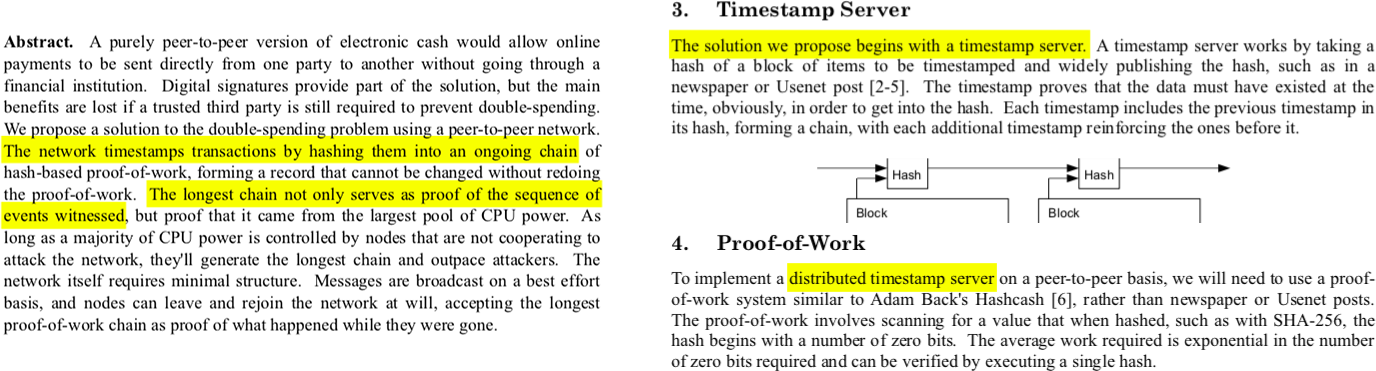
\includegraphics{assets/images/bitcoin-whitepaper-timestamp-wide.png}
  \caption{Excerpts from the whitepaper. Did someone say timechain?}
  \label{fig:bitcoin-whitepaper-timestamp-wide}
\end{figure}

When I first learned how Bitcoin works I also thought that proof-of-work
is inefficient and wasteful. After a while, I started to shift my
perspective on Bitcoin's energy consumption~\cite{gigi:energy}. It seems that
proof-of-work is still widely misunderstood today, in the year 10 AB
(after Bitcoin).

Since the problems to be solved in proof-of-work are made up, many
people seem to believe that it is \textit{useless} work. If the focus is purely
on the computation, this is an understandable conclusion. But Bitcoin
isn't about computation. It is about \textit{independently agreeing on the
order of things.}

Proof-of-work is a system in which everyone can validate what happened
and in what order it happened. This independent validation is what leads
to consensus, an individual agreement by multiple parties about who owns
what.

In a radically decentralized environment, we don't have the luxury of absolute
time. Any clock would introduce a trusted third party, a central point in the
system which had to be relied upon and could be attacked. \enquote{Timing is the root
problem,} as Grisha Trubetskoy points out~\cite{pow-clock}. And Satoshi
brilliantly solved this problem by implementing a decentralized clock via a
proof-of-work blockchain. Everyone agrees beforehand that the chain with the
most cumulative work is the source of truth. It is per definition what actually
happened. This agreement is what is now known as Nakamoto consensus.

\begin{quotation}\begin{samepage}
\enquote{The network timestamps transactions by hashing them into an ongoing
chain which serves as proof of the sequence of events witnessed}
\begin{flushright} -- Satoshi Nakamoto\footnote{Satoshi Nakamoto, the Bitcoin whitepaper~\cite{whitepaper}}
\end{flushright}\end{samepage}\end{quotation}

Without a consistent way to tell the time, there is no consistent way to
tell before from after. Reliable ordering is impossible. As mentioned
above, Nakamoto consensus is Bitcoin's way to consistently tell the
time. The system's incentive structure produces a probabilistic,
decentralized clock, by utilizing both greed and self-interest of
competing participants. The fact that this clock is imprecise is
irrelevant because the order of events is eventually unambiguous and can
be verified by anyone.

Thanks to proof-of-work, both the work \textit{and} the validation of the work
are radically decentralized. Everyone can join and leave at will, and
everyone can validate everything at all times. Not only that, but
everyone can validate the state of the system \textit{individually}, without
having to rely on anyone else for validation.

Understanding proof-of-work takes time. It is often counter-intuitive,
and while the rules are simple, they lead to quite complex phenomena.
For me, shifting my perspective on mining helped. Useful, not useless.
Validation, not computation. Time, not blocks.

\paragraph{Bitcoin taught me that telling the time is tricky, especially if you are
decentralized.}

% ---
%
% #### Through the Looking-Glass
%
% - [Bitcoin's Energy Consumption: A shift in perspective][energy]
%
% #### Down the Rabbit Hole
%
% - [Blockchain Proof-of-Work Is a Decentralized Clock][points out] by Gregory Trubetskoy
% - [The Anatomy of Proof-of-Work][pow-anatomy] by Hugo Nguyen
% - [PoW is efficient][pow-efficient] by Dan Held
% - [Mining][bw-mining], [Controlled supply][bw-supply] on the Bitcoin Wiki
%
% [points out]: https://grisha.org/blog/2018/01/23/explaining-proof-of-work/
% [energy]: 
% [whitepaper]: https://bitcoin.org/bitcoin.pdf
%
% [pow-efficient]: https://blog.picks.co/pow-is-efficient-aa3d442754d3
% [pow-anatomy]: https://bitcointechtalk.com/the-anatomy-of-proof-of-work-98c85b6f6667
% [bw-mining]: https://en.bitcoin.it/wiki/Mining
% [bw-supply]: https://en.bitcoin.it/wiki/Controlled_supply
%
% <!-- Wikipedia -->
% [alice]: https://en.wikipedia.org/wiki/Alice%27s_Adventures_in_Wonderland
% [carroll]: https://en.wikipedia.org/wiki/Lewis_Carroll
